\documentclass[1p]{elsarticle_modified}
%\bibliographystyle{elsarticle-num}

%\usepackage[colorlinks]{hyperref}
%\usepackage{abbrmath_seonhwa} %\Abb, \Ascr, \Acal ,\Abf, \Afrak
\usepackage{amsfonts}
\usepackage{amssymb}
\usepackage{amsmath}
\usepackage{amsthm}
\usepackage{scalefnt}
\usepackage{amsbsy}
\usepackage{kotex}
\usepackage{caption}
\usepackage{subfig}
\usepackage{color}
\usepackage{graphicx}
\usepackage{xcolor} %% white, black, red, green, blue, cyan, magenta, yellow
\usepackage{float}
\usepackage{setspace}
\usepackage{hyperref}

\usepackage{tikz}
\usetikzlibrary{arrows}

\usepackage{multirow}
\usepackage{array} % fixed length table
\usepackage{hhline}

%%%%%%%%%%%%%%%%%%%%%
\makeatletter
\renewcommand*\env@matrix[1][\arraystretch]{%
	\edef\arraystretch{#1}%
	\hskip -\arraycolsep
	\let\@ifnextchar\new@ifnextchar
	\array{*\c@MaxMatrixCols c}}
\makeatother %https://tex.stackexchange.com/questions/14071/how-can-i-increase-the-line-spacing-in-a-matrix
%%%%%%%%%%%%%%%

\usepackage[normalem]{ulem}

\newcommand{\msout}[1]{\ifmmode\text{\sout{\ensuremath{#1}}}\else\sout{#1}\fi}
%SOURCE: \msout is \stkout macro in https://tex.stackexchange.com/questions/20609/strikeout-in-math-mode

\newcommand{\cancel}[1]{
	\ifmmode
	{\color{red}\msout{#1}}
	\else
	{\color{red}\sout{#1}}
	\fi
}

\newcommand{\add}[1]{
	{\color{blue}\uwave{#1}}
}

\newcommand{\replace}[2]{
	\ifmmode
	{\color{red}\msout{#1}}{\color{blue}\uwave{#2}}
	\else
	{\color{red}\sout{#1}}{\color{blue}\uwave{#2}}
	\fi
}

\newcommand{\Sol}{\mathcal{S}} %segment
\newcommand{\D}{D} %diagram
\newcommand{\A}{\mathcal{A}} %arc


%%%%%%%%%%%%%%%%%%%%%%%%%%%%%5 test

\def\sl{\operatorname{\textup{SL}}(2,\Cbb)}
\def\psl{\operatorname{\textup{PSL}}(2,\Cbb)}
\def\quan{\mkern 1mu \triangleright \mkern 1mu}

\theoremstyle{definition}
\newtheorem{thm}{Theorem}[section]
\newtheorem{prop}[thm]{Proposition}
\newtheorem{lem}[thm]{Lemma}
\newtheorem{ques}[thm]{Question}
\newtheorem{cor}[thm]{Corollary}
\newtheorem{defn}[thm]{Definition}
\newtheorem{exam}[thm]{Example}
\newtheorem{rmk}[thm]{Remark}
\newtheorem{alg}[thm]{Algorithm}

\newcommand{\I}{\sqrt{-1}}
\begin{document}

%\begin{frontmatter}
%
%\title{Boundary parabolic representations of knots up to 8 crossings}
%
%%% Group authors per affiliation:
%\author{Yunhi Cho} 
%\address{Department of Mathematics, University of Seoul, Seoul, Korea}
%\ead{yhcho@uos.ac.kr}
%
%
%\author{Seonhwa Kim} %\fnref{s_kim}}
%\address{Center for Geometry and Physics, Institute for Basic Science, Pohang, 37673, Korea}
%\ead{ryeona17@ibs.re.kr}
%
%\author{Hyuk Kim}
%\address{Department of Mathematical Sciences, Seoul National University, Seoul 08826, Korea}
%\ead{hyukkim@snu.ac.kr}
%
%\author{Seokbeom Yoon}
%\address{Department of Mathematical Sciences, Seoul National University, Seoul, 08826,  Korea}
%\ead{sbyoon15@snu.ac.kr}
%
%\begin{abstract}
%We find all boundary parabolic representation of knots up to 8 crossings.
%
%\end{abstract}
%\begin{keyword}
%    \MSC[2010] 57M25 
%\end{keyword}
%
%\end{frontmatter}

%\linenumbers
%\tableofcontents
%
\newcommand\colored[1]{\textcolor{white}{\rule[-0.35ex]{0.8em}{1.4ex}}\kern-0.8em\color{red} #1}%
%\newcommand\colored[1]{\textcolor{white}{ #1}\kern-2.17ex	\textcolor{white}{ #1}\kern-1.81ex	\textcolor{white}{ #1}\kern-2.15ex\color{red}#1	}

{\Large $\underline{12a_{0611}~(K12a_{0611})}$}

\setlength{\tabcolsep}{10pt}
\renewcommand{\arraystretch}{1.6}
\vspace{1cm}\begin{tabular}{m{100pt}>{\centering\arraybackslash}m{274pt}}
\multirow{5}{120pt}{
	\centering
	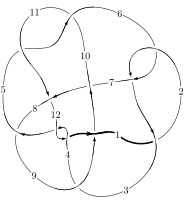
\includegraphics[width=112pt]{../../../GIT/diagram.site/Diagrams/png/1412_12a_0611.png}\\
\ \ \ A knot diagram\footnotemark}&
\allowdisplaybreaks
\textbf{Linearized knot diagam} \\
\cline{2-2}
 &
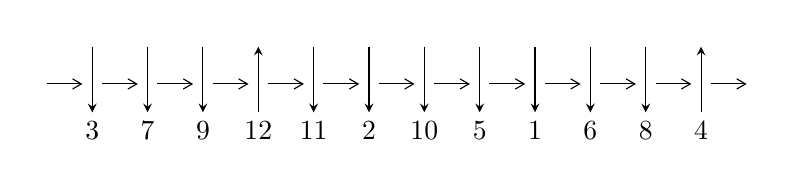
\begin{tikzpicture}[x=20pt, y=17pt]
	% nodes
	\node (C0) at (0, 0) {};
	\node (C1) at (1, 0) {};
	\node (C1U) at (1, +1) {};
	\node (C1D) at (1, -1) {3};

	\node (C2) at (2, 0) {};
	\node (C2U) at (2, +1) {};
	\node (C2D) at (2, -1) {7};

	\node (C3) at (3, 0) {};
	\node (C3U) at (3, +1) {};
	\node (C3D) at (3, -1) {9};

	\node (C4) at (4, 0) {};
	\node (C4U) at (4, +1) {};
	\node (C4D) at (4, -1) {12};

	\node (C5) at (5, 0) {};
	\node (C5U) at (5, +1) {};
	\node (C5D) at (5, -1) {11};

	\node (C6) at (6, 0) {};
	\node (C6U) at (6, +1) {};
	\node (C6D) at (6, -1) {2};

	\node (C7) at (7, 0) {};
	\node (C7U) at (7, +1) {};
	\node (C7D) at (7, -1) {10};

	\node (C8) at (8, 0) {};
	\node (C8U) at (8, +1) {};
	\node (C8D) at (8, -1) {5};

	\node (C9) at (9, 0) {};
	\node (C9U) at (9, +1) {};
	\node (C9D) at (9, -1) {1};

	\node (C10) at (10, 0) {};
	\node (C10U) at (10, +1) {};
	\node (C10D) at (10, -1) {6};

	\node (C11) at (11, 0) {};
	\node (C11U) at (11, +1) {};
	\node (C11D) at (11, -1) {8};

	\node (C12) at (12, 0) {};
	\node (C12U) at (12, +1) {};
	\node (C12D) at (12, -1) {4};
	\node (C13) at (13, 0) {};

	% arrows
	\draw[->,>={angle 60}]
	(C0) edge (C1) (C1) edge (C2) (C2) edge (C3) (C3) edge (C4) (C4) edge (C5) (C5) edge (C6) (C6) edge (C7) (C7) edge (C8) (C8) edge (C9) (C9) edge (C10) (C10) edge (C11) (C11) edge (C12) (C12) edge (C13) ;	\draw[->,>=stealth]
	(C1U) edge (C1D) (C2U) edge (C2D) (C3U) edge (C3D) (C4D) edge (C4U) (C5U) edge (C5D) (C6U) edge (C6D) (C7U) edge (C7D) (C8U) edge (C8D) (C9U) edge (C9D) (C10U) edge (C10D) (C11U) edge (C11D) (C12D) edge (C12U) ;
	\end{tikzpicture} \\
\hhline{~~} \\& 
\textbf{Solving Sequence} \\ \cline{2-2} 
 &
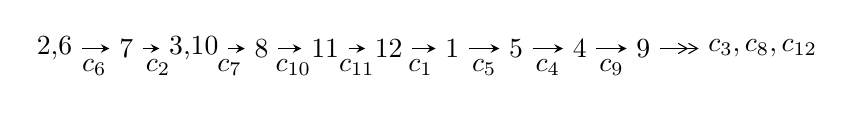
\begin{tikzpicture}[x=23pt, y=7pt]
	% node
	\node (A0) at (-1/8, 0) {2,6};
	\node (A1) at (1, 0) {7};
	\node (A2) at (33/16, 0) {3,10};
	\node (A3) at (25/8, 0) {8};
	\node (A4) at (33/8, 0) {11};
	\node (A5) at (41/8, 0) {12};
	\node (A6) at (49/8, 0) {1};
	\node (A7) at (57/8, 0) {5};
	\node (A8) at (65/8, 0) {4};
	\node (A9) at (73/8, 0) {9};
	\node (C1) at (1/2, -1) {$c_{6}$};
	\node (C2) at (3/2, -1) {$c_{2}$};
	\node (C3) at (21/8, -1) {$c_{7}$};
	\node (C4) at (29/8, -1) {$c_{10}$};
	\node (C5) at (37/8, -1) {$c_{11}$};
	\node (C6) at (45/8, -1) {$c_{1}$};
	\node (C7) at (53/8, -1) {$c_{5}$};
	\node (C8) at (61/8, -1) {$c_{4}$};
	\node (C9) at (69/8, -1) {$c_{9}$};
	\node (A10) at (11, 0) {$c_{3},c_{8},c_{12}$};

	% edge
	\draw[->,>=stealth]	
	(A0) edge (A1) (A1) edge (A2) (A2) edge (A3) (A3) edge (A4) (A4) edge (A5) (A5) edge (A6) (A6) edge (A7) (A7) edge (A8) (A8) edge (A9) ;
	\draw[->>,>={angle 60}]	
	(A9) edge (A10);
\end{tikzpicture} \\ 

\end{tabular} \\

\footnotetext{
The image of knot diagram is generated by the software ``\textbf{Draw programme}" developed by Andrew Bartholomew(\url{http://www.layer8.co.uk/maths/draw/index.htm\#Running-draw}), where we modified some parts for our purpose(\url{https://github.com/CATsTAILs/LinksPainter}).
}\phantom \\ \newline 
\centering \textbf{Ideals for irreducible components\footnotemark of $X_{\text{par}}$} 
 
\begin{align*}
I^u_{1}&=\langle 
9.13312\times10^{361} u^{148}-1.51853\times10^{362} u^{147}+\cdots+8.68141\times10^{362} b-9.20259\times10^{363},\\
\phantom{I^u_{1}}&\phantom{= \langle  }4.19476\times10^{364} u^{148}-8.08613\times10^{364} u^{147}+\cdots+1.61474\times10^{365} a+3.78553\times10^{366},\\
\phantom{I^u_{1}}&\phantom{= \langle  }u^{149}-2 u^{148}+\cdots+105 u+93\rangle \\
I^u_{2}&=\langle 
54 u^{27}-138 u^{26}+\cdots+13 b-174,\;-36 u^{27}+40 u^{26}+\cdots+13 a+25,\;u^{28}-2 u^{27}+\cdots-3 u+1\rangle \\
I^u_{3}&=\langle 
b- a-1,\;a^3+4 a^2+7 a+5,\;u+1\rangle \\
\\
\end{align*}
\raggedright * 3 irreducible components of $\dim_{\mathbb{C}}=0$, with total 180 representations.\\
\footnotetext{All coefficients of polynomials are rational numbers. But the coefficients are sometimes approximated in decimal forms when there is not enough margin.}
\newpage
\renewcommand{\arraystretch}{1}
\centering \section*{I. $I^u_{1}= \langle 9.13\times10^{361} u^{148}-1.52\times10^{362} u^{147}+\cdots+8.68\times10^{362} b-9.20\times10^{363},\;4.19\times10^{364} u^{148}-8.09\times10^{364} u^{147}+\cdots+1.61\times10^{365} a+3.79\times10^{366},\;u^{149}-2 u^{148}+\cdots+105 u+93 \rangle$}
\flushleft \textbf{(i) Arc colorings}\\
\begin{tabular}{m{7pt} m{180pt} m{7pt} m{180pt} }
\flushright $a_{2}=$&$\begin{pmatrix}0\\u\end{pmatrix}$ \\
\flushright $a_{6}=$&$\begin{pmatrix}1\\0\end{pmatrix}$ \\
\flushright $a_{7}=$&$\begin{pmatrix}1\\u^2\end{pmatrix}$ \\
\flushright $a_{3}=$&$\begin{pmatrix}- u\\- u^3+u\end{pmatrix}$ \\
\flushright $a_{10}=$&$\begin{pmatrix}-0.259779 u^{148}+0.500769 u^{147}+\cdots-15.1768 u-23.4436\\-0.105203 u^{148}+0.174917 u^{147}+\cdots+90.1082 u+10.6003\end{pmatrix}$ \\
\flushright $a_{8}=$&$\begin{pmatrix}0.00360016 u^{148}-0.0517405 u^{147}+\cdots+141.346 u+47.5754\\-0.0929461 u^{148}+0.00270813 u^{147}+\cdots+16.2736 u-0.477362\end{pmatrix}$ \\
\flushright $a_{11}=$&$\begin{pmatrix}-0.154576 u^{148}+0.325852 u^{147}+\cdots-105.285 u-34.0439\\-0.105203 u^{148}+0.174917 u^{147}+\cdots+90.1082 u+10.6003\end{pmatrix}$ \\
\flushright $a_{12}=$&$\begin{pmatrix}0.0468139 u^{148}+0.0510239 u^{147}+\cdots+61.5072 u+23.2256\\-0.0175283 u^{148}-0.125085 u^{147}+\cdots+5.97799 u-1.90294\end{pmatrix}$ \\
\flushright $a_{1}=$&$\begin{pmatrix}u^3\\u^5- u^3+u\end{pmatrix}$ \\
\flushright $a_{5}=$&$\begin{pmatrix}0.0459520 u^{148}+0.0568612 u^{147}+\cdots-77.0611 u-35.6329\\0.00726844 u^{148}+0.0815554 u^{147}+\cdots-46.9332 u-22.2944\end{pmatrix}$ \\
\flushright $a_{4}=$&$\begin{pmatrix}0.0162594 u^{148}-0.201415 u^{147}+\cdots-20.2519 u+16.5162\\0.223761 u^{148}-0.411051 u^{147}+\cdots-58.8642 u-17.8281\end{pmatrix}$ \\
\flushright $a_{9}=$&$\begin{pmatrix}-0.325654 u^{148}+0.818894 u^{147}+\cdots-17.3532 u-13.0768\\-0.102726 u^{148}+0.0936566 u^{147}+\cdots+97.3876 u+9.56960\end{pmatrix}$\\&\end{tabular}
\flushleft \textbf{(ii) Obstruction class $= -1$}\\~\\
\flushleft \textbf{(iii) Cusp Shapes $= -0.688479 u^{148}+1.43565 u^{147}+\cdots+375.146 u+114.095$}\\~\\
\newpage\renewcommand{\arraystretch}{1}
\flushleft \textbf{(iv) u-Polynomials at the component}\newline \\
\begin{tabular}{m{50pt}|m{274pt}}
Crossings & \hspace{64pt}u-Polynomials at each crossing \\
\hline $$\begin{aligned}c_{1}\end{aligned}$$&$\begin{aligned}
&u^{149}+56 u^{148}+\cdots+296535 u+8649
\end{aligned}$\\
\hline $$\begin{aligned}c_{2},c_{6}\end{aligned}$$&$\begin{aligned}
&u^{149}-2 u^{148}+\cdots+105 u+93
\end{aligned}$\\
\hline $$\begin{aligned}c_{3}\end{aligned}$$&$\begin{aligned}
&u^{149}- u^{148}+\cdots+2245 u+181
\end{aligned}$\\
\hline $$\begin{aligned}c_{4},c_{12}\end{aligned}$$&$\begin{aligned}
&u^{149}+6 u^{148}+\cdots+79 u+1
\end{aligned}$\\
\hline $$\begin{aligned}c_{5},c_{10}\end{aligned}$$&$\begin{aligned}
&u^{149}+2 u^{148}+\cdots-3779 u+113
\end{aligned}$\\
\hline $$\begin{aligned}c_{7}\end{aligned}$$&$\begin{aligned}
&u^{149}+10 u^{148}+\cdots+30325383 u+3181516
\end{aligned}$\\
\hline $$\begin{aligned}c_{8}\end{aligned}$$&$\begin{aligned}
&u^{149}+5 u^{148}+\cdots+1104 u+48
\end{aligned}$\\
\hline $$\begin{aligned}c_{9}\end{aligned}$$&$\begin{aligned}
&u^{149}+8 u^{148}+\cdots+15407 u+3844
\end{aligned}$\\
\hline $$\begin{aligned}c_{11}\end{aligned}$$&$\begin{aligned}
&u^{149}-3 u^{148}+\cdots+7 u+1
\end{aligned}$\\
\hline
\end{tabular}\\~\\
\newpage\renewcommand{\arraystretch}{1}
\flushleft \textbf{(v) Riley Polynomials at the component}\newline \\
\begin{tabular}{m{50pt}|m{274pt}}
Crossings & \hspace{64pt}Riley Polynomials at each crossing \\
\hline $$\begin{aligned}c_{1}\end{aligned}$$&$\begin{aligned}
&y^{149}+72 y^{148}+\cdots+8853694299 y-74805201
\end{aligned}$\\
\hline $$\begin{aligned}c_{2},c_{6}\end{aligned}$$&$\begin{aligned}
&y^{149}-56 y^{148}+\cdots+296535 y-8649
\end{aligned}$\\
\hline $$\begin{aligned}c_{3}\end{aligned}$$&$\begin{aligned}
&y^{149}-3 y^{148}+\cdots+466517 y-32761
\end{aligned}$\\
\hline $$\begin{aligned}c_{4},c_{12}\end{aligned}$$&$\begin{aligned}
&y^{149}+110 y^{148}+\cdots+709 y-1
\end{aligned}$\\
\hline $$\begin{aligned}c_{5},c_{10}\end{aligned}$$&$\begin{aligned}
&y^{149}+114 y^{148}+\cdots-5658461 y-12769
\end{aligned}$\\
\hline $$\begin{aligned}c_{7}\end{aligned}$$&$\begin{aligned}
&y^{149}+40 y^{148}+\cdots+174252360290745 y-10122044058256
\end{aligned}$\\
\hline $$\begin{aligned}c_{8}\end{aligned}$$&$\begin{aligned}
&y^{149}+7 y^{148}+\cdots-180096 y-2304
\end{aligned}$\\
\hline $$\begin{aligned}c_{9}\end{aligned}$$&$\begin{aligned}
&y^{149}-20 y^{148}+\cdots+533917185 y-14776336
\end{aligned}$\\
\hline $$\begin{aligned}c_{11}\end{aligned}$$&$\begin{aligned}
&y^{149}-5 y^{148}+\cdots-2703 y-1
\end{aligned}$\\
\hline
\end{tabular}\\~\\
\newpage\flushleft \textbf{(vi) Complex Volumes and Cusp Shapes}
$$\begin{array}{c|c|c}  
\text{Solutions to }I^u_{1}& \I (\text{vol} + \sqrt{-1}CS) & \text{Cusp shape}\\
 \hline 
\begin{aligned}
u &= \phantom{-}0.968469 + 0.235445 I \\
a &= \phantom{-}0.383733 + 0.623501 I \\
b &= \phantom{-}0.403217 - 0.178671 I\end{aligned}
 & -4.22553 + 2.20818 I & \phantom{-0.000000 } 0 \\ \hline\begin{aligned}
u &= \phantom{-}0.968469 - 0.235445 I \\
a &= \phantom{-}0.383733 - 0.623501 I \\
b &= \phantom{-}0.403217 + 0.178671 I\end{aligned}
 & -4.22553 - 2.20818 I & \phantom{-0.000000 } 0 \\ \hline\begin{aligned}
u &= -0.640300 + 0.772807 I \\
a &= \phantom{-}0.803379 - 0.344187 I \\
b &= \phantom{-}0.331748 + 1.047570 I\end{aligned}
 & -0.04142 - 4.05732 I & \phantom{-0.000000 } 0 \\ \hline\begin{aligned}
u &= -0.640300 - 0.772807 I \\
a &= \phantom{-}0.803379 + 0.344187 I \\
b &= \phantom{-}0.331748 - 1.047570 I\end{aligned}
 & -0.04142 + 4.05732 I & \phantom{-0.000000 } 0 \\ \hline\begin{aligned}
u &= \phantom{-}0.699565 + 0.704970 I \\
a &= \phantom{-}1.069920 - 0.219227 I \\
b &= \phantom{-}0.805668 + 0.420642 I\end{aligned}
 & -1.96563 - 0.24185 I & \phantom{-0.000000 } 0 \\ \hline\begin{aligned}
u &= \phantom{-}0.699565 - 0.704970 I \\
a &= \phantom{-}1.069920 + 0.219227 I \\
b &= \phantom{-}0.805668 - 0.420642 I\end{aligned}
 & -1.96563 + 0.24185 I & \phantom{-0.000000 } 0 \\ \hline\begin{aligned}
u &= -0.827837 + 0.589865 I \\
a &= -1.04994 - 1.25770 I \\
b &= -1.159570 - 0.123204 I\end{aligned}
 & -0.36402 + 4.16944 I & \phantom{-0.000000 } 0 \\ \hline\begin{aligned}
u &= -0.827837 - 0.589865 I \\
a &= -1.04994 + 1.25770 I \\
b &= -1.159570 + 0.123204 I\end{aligned}
 & -0.36402 - 4.16944 I & \phantom{-0.000000 } 0 \\ \hline\begin{aligned}
u &= -0.824013 + 0.527857 I \\
a &= \phantom{-}0.747555 + 0.400726 I \\
b &= \phantom{-}0.832215 + 0.164773 I\end{aligned}
 & -0.365322 + 0.476907 I & \phantom{-0.000000 } 0 \\ \hline\begin{aligned}
u &= -0.824013 - 0.527857 I \\
a &= \phantom{-}0.747555 - 0.400726 I \\
b &= \phantom{-}0.832215 - 0.164773 I\end{aligned}
 & -0.365322 - 0.476907 I & \phantom{-0.000000 } 0\\
 \hline 
 \end{array}$$\newpage$$\begin{array}{c|c|c}  
\text{Solutions to }I^u_{1}& \I (\text{vol} + \sqrt{-1}CS) & \text{Cusp shape}\\
 \hline 
\begin{aligned}
u &= -0.526498 + 0.875430 I \\
a &= \phantom{-}0.107153 + 0.304455 I \\
b &= -0.590870 - 0.185138 I\end{aligned}
 & -2.59432 + 4.59273 I & \phantom{-0.000000 } 0 \\ \hline\begin{aligned}
u &= -0.526498 - 0.875430 I \\
a &= \phantom{-}0.107153 - 0.304455 I \\
b &= -0.590870 + 0.185138 I\end{aligned}
 & -2.59432 - 4.59273 I & \phantom{-0.000000 } 0 \\ \hline\begin{aligned}
u &= \phantom{-}0.714566 + 0.734165 I \\
a &= \phantom{-}0.286501 - 0.302094 I \\
b &= -0.091309 + 1.350030 I\end{aligned}
 & \phantom{-}4.81717 - 1.31981 I & \phantom{-0.000000 } 0 \\ \hline\begin{aligned}
u &= \phantom{-}0.714566 - 0.734165 I \\
a &= \phantom{-}0.286501 + 0.302094 I \\
b &= -0.091309 - 1.350030 I\end{aligned}
 & \phantom{-}4.81717 + 1.31981 I & \phantom{-0.000000 } 0 \\ \hline\begin{aligned}
u &= -0.984794 + 0.282534 I \\
a &= -1.53905 - 1.13501 I \\
b &= -0.413838 + 0.070302 I\end{aligned}
 & -7.05553 + 0.84983 I & \phantom{-0.000000 } 0 \\ \hline\begin{aligned}
u &= -0.984794 - 0.282534 I \\
a &= -1.53905 + 1.13501 I \\
b &= -0.413838 - 0.070302 I\end{aligned}
 & -7.05553 - 0.84983 I & \phantom{-0.000000 } 0 \\ \hline\begin{aligned}
u &= -0.825747 + 0.609487 I \\
a &= \phantom{-}0.918486 + 0.460716 I \\
b &= \phantom{-}0.950081 - 0.016109 I\end{aligned}
 & -0.392806 + 0.526558 I & \phantom{-0.000000 } 0 \\ \hline\begin{aligned}
u &= -0.825747 - 0.609487 I \\
a &= \phantom{-}0.918486 - 0.460716 I \\
b &= \phantom{-}0.950081 + 0.016109 I\end{aligned}
 & -0.392806 - 0.526558 I & \phantom{-0.000000 } 0 \\ \hline\begin{aligned}
u &= \phantom{-}0.860642 + 0.568093 I \\
a &= -1.84264 + 0.93586 I \\
b &= -0.07523 - 1.64011 I\end{aligned}
 & -1.09307 - 2.26272 I & \phantom{-0.000000 } 0 \\ \hline\begin{aligned}
u &= \phantom{-}0.860642 - 0.568093 I \\
a &= -1.84264 - 0.93586 I \\
b &= -0.07523 + 1.64011 I\end{aligned}
 & -1.09307 + 2.26272 I & \phantom{-0.000000 } 0\\
 \hline 
 \end{array}$$\newpage$$\begin{array}{c|c|c}  
\text{Solutions to }I^u_{1}& \I (\text{vol} + \sqrt{-1}CS) & \text{Cusp shape}\\
 \hline 
\begin{aligned}
u &= -0.803588 + 0.649713 I \\
a &= -0.419576 - 0.160156 I \\
b &= \phantom{-}0.42860 + 1.59171 I\end{aligned}
 & \phantom{-}6.18278 - 0.66023 I & \phantom{-0.000000 } 0 \\ \hline\begin{aligned}
u &= -0.803588 - 0.649713 I \\
a &= -0.419576 + 0.160156 I \\
b &= \phantom{-}0.42860 - 1.59171 I\end{aligned}
 & \phantom{-}6.18278 + 0.66023 I & \phantom{-0.000000 } 0 \\ \hline\begin{aligned}
u &= -0.515537 + 0.811811 I \\
a &= -0.195761 - 0.402466 I \\
b &= -1.030710 - 0.273295 I\end{aligned}
 & -2.71841 - 8.19281 I & \phantom{-0.000000 } 0 \\ \hline\begin{aligned}
u &= -0.515537 - 0.811811 I \\
a &= -0.195761 + 0.402466 I \\
b &= -1.030710 + 0.273295 I\end{aligned}
 & -2.71841 + 8.19281 I & \phantom{-0.000000 } 0 \\ \hline\begin{aligned}
u &= \phantom{-}0.749923 + 0.720134 I \\
a &= \phantom{-}0.1159100 + 0.0441175 I \\
b &= \phantom{-}0.50626 - 1.40796 I\end{aligned}
 & \phantom{-}4.11574 + 5.05670 I & \phantom{-0.000000 } 0 \\ \hline\begin{aligned}
u &= \phantom{-}0.749923 - 0.720134 I \\
a &= \phantom{-}0.1159100 - 0.0441175 I \\
b &= \phantom{-}0.50626 + 1.40796 I\end{aligned}
 & \phantom{-}4.11574 - 5.05670 I & \phantom{-0.000000 } 0 \\ \hline\begin{aligned}
u &= \phantom{-}0.843931 + 0.621675 I \\
a &= -0.75324 - 1.33079 I \\
b &= \phantom{-}0.016408 + 1.258060 I\end{aligned}
 & \phantom{-}2.04435 - 7.80962 I & \phantom{-0.000000 } 0 \\ \hline\begin{aligned}
u &= \phantom{-}0.843931 - 0.621675 I \\
a &= -0.75324 + 1.33079 I \\
b &= \phantom{-}0.016408 - 1.258060 I\end{aligned}
 & \phantom{-}2.04435 + 7.80962 I & \phantom{-0.000000 } 0 \\ \hline\begin{aligned}
u &= \phantom{-}0.614857 + 0.707173 I \\
a &= \phantom{-}0.657947 - 0.495014 I \\
b &= -0.0235396 - 0.0419572 I\end{aligned}
 & \phantom{-}3.04411 - 0.49008 I & \phantom{-0.000000 } 0 \\ \hline\begin{aligned}
u &= \phantom{-}0.614857 - 0.707173 I \\
a &= \phantom{-}0.657947 + 0.495014 I \\
b &= -0.0235396 + 0.0419572 I\end{aligned}
 & \phantom{-}3.04411 + 0.49008 I & \phantom{-0.000000 } 0\\
 \hline 
 \end{array}$$\newpage$$\begin{array}{c|c|c}  
\text{Solutions to }I^u_{1}& \I (\text{vol} + \sqrt{-1}CS) & \text{Cusp shape}\\
 \hline 
\begin{aligned}
u &= \phantom{-}1.061270 + 0.060244 I \\
a &= -1.56436 - 1.28089 I \\
b &= -0.363717 - 0.882385 I\end{aligned}
 & -5.88809 - 3.57709 I & \phantom{-0.000000 } 0 \\ \hline\begin{aligned}
u &= \phantom{-}1.061270 - 0.060244 I \\
a &= -1.56436 + 1.28089 I \\
b &= -0.363717 + 0.882385 I\end{aligned}
 & -5.88809 + 3.57709 I & \phantom{-0.000000 } 0 \\ \hline\begin{aligned}
u &= -1.038870 + 0.233922 I \\
a &= \phantom{-}1.79709 - 0.52310 I \\
b &= \phantom{-}0.82029 - 1.51104 I\end{aligned}
 & -3.99947 - 0.27695 I & \phantom{-0.000000 } 0 \\ \hline\begin{aligned}
u &= -1.038870 - 0.233922 I \\
a &= \phantom{-}1.79709 + 0.52310 I \\
b &= \phantom{-}0.82029 + 1.51104 I\end{aligned}
 & -3.99947 + 0.27695 I & \phantom{-0.000000 } 0 \\ \hline\begin{aligned}
u &= \phantom{-}0.911782 + 0.199111 I \\
a &= -1.76696 + 0.52732 I \\
b &= -0.383269 - 0.466773 I\end{aligned}
 & -3.26613 - 0.66224 I & \phantom{-0.000000 } 0 \\ \hline\begin{aligned}
u &= \phantom{-}0.911782 - 0.199111 I \\
a &= -1.76696 - 0.52732 I \\
b &= -0.383269 + 0.466773 I\end{aligned}
 & -3.26613 + 0.66224 I & \phantom{-0.000000 } 0 \\ \hline\begin{aligned}
u &= -0.833825 + 0.667958 I \\
a &= \phantom{-}0.038318 + 1.117750 I \\
b &= \phantom{-}0.014891 - 1.310330 I\end{aligned}
 & \phantom{-}6.50540 + 4.42575 I & \phantom{-0.000000 } 0 \\ \hline\begin{aligned}
u &= -0.833825 - 0.667958 I \\
a &= \phantom{-}0.038318 - 1.117750 I \\
b &= \phantom{-}0.014891 + 1.310330 I\end{aligned}
 & \phantom{-}6.50540 - 4.42575 I & \phantom{-0.000000 } 0 \\ \hline\begin{aligned}
u &= \phantom{-}0.500409 + 0.945676 I \\
a &= \phantom{-}0.234386 + 0.299924 I \\
b &= \phantom{-}0.093036 - 1.298950 I\end{aligned}
 & \phantom{-}4.79305 + 4.31248 I & \phantom{-0.000000 } 0 \\ \hline\begin{aligned}
u &= \phantom{-}0.500409 - 0.945676 I \\
a &= \phantom{-}0.234386 - 0.299924 I \\
b &= \phantom{-}0.093036 + 1.298950 I\end{aligned}
 & \phantom{-}4.79305 - 4.31248 I & \phantom{-0.000000 } 0\\
 \hline 
 \end{array}$$\newpage$$\begin{array}{c|c|c}  
\text{Solutions to }I^u_{1}& \I (\text{vol} + \sqrt{-1}CS) & \text{Cusp shape}\\
 \hline 
\begin{aligned}
u &= \phantom{-}0.867238 + 0.630962 I \\
a &= \phantom{-}2.95975 - 0.34566 I \\
b &= \phantom{-}0.014521 + 1.147190 I\end{aligned}
 & \phantom{-}1.96855 + 2.90153 I & \phantom{-0.000000 } 0 \\ \hline\begin{aligned}
u &= \phantom{-}0.867238 - 0.630962 I \\
a &= \phantom{-}2.95975 + 0.34566 I \\
b &= \phantom{-}0.014521 - 1.147190 I\end{aligned}
 & \phantom{-}1.96855 - 2.90153 I & \phantom{-0.000000 } 0 \\ \hline\begin{aligned}
u &= \phantom{-}0.567008 + 0.718904 I \\
a &= \phantom{-}0.505387 + 0.378998 I \\
b &= \phantom{-}0.278342 - 1.278840 I\end{aligned}
 & \phantom{-}3.89964 + 3.17460 I & \phantom{-0.000000 } 0 \\ \hline\begin{aligned}
u &= \phantom{-}0.567008 - 0.718904 I \\
a &= \phantom{-}0.505387 - 0.378998 I \\
b &= \phantom{-}0.278342 + 1.278840 I\end{aligned}
 & \phantom{-}3.89964 - 3.17460 I & \phantom{-0.000000 } 0 \\ \hline\begin{aligned}
u &= \phantom{-}0.238710 + 1.060760 I \\
a &= -0.143371 + 0.495180 I \\
b &= -0.307023 - 1.200370 I\end{aligned}
 & \phantom{-}0.56832 - 8.02901 I & \phantom{-0.000000 } 0 \\ \hline\begin{aligned}
u &= \phantom{-}0.238710 - 1.060760 I \\
a &= -0.143371 - 0.495180 I \\
b &= -0.307023 + 1.200370 I\end{aligned}
 & \phantom{-}0.56832 + 8.02901 I & \phantom{-0.000000 } 0 \\ \hline\begin{aligned}
u &= -0.819821 + 0.379396 I \\
a &= \phantom{-}0.067222 - 1.404120 I \\
b &= -0.239208 - 1.269010 I\end{aligned}
 & -2.14758 + 1.53177 I & \phantom{-0.000000 } 0 \\ \hline\begin{aligned}
u &= -0.819821 - 0.379396 I \\
a &= \phantom{-}0.067222 + 1.404120 I \\
b &= -0.239208 + 1.269010 I\end{aligned}
 & -2.14758 - 1.53177 I & \phantom{-0.000000 } 0 \\ \hline\begin{aligned}
u &= -0.873328 + 0.666062 I \\
a &= \phantom{-}2.19574 + 0.68805 I \\
b &= \phantom{-}0.040551 - 1.210860 I\end{aligned}
 & \phantom{-}6.38250 + 0.73820 I & \phantom{-0.000000 } 0 \\ \hline\begin{aligned}
u &= -0.873328 - 0.666062 I \\
a &= \phantom{-}2.19574 - 0.68805 I \\
b &= \phantom{-}0.040551 + 1.210860 I\end{aligned}
 & \phantom{-}6.38250 - 0.73820 I & \phantom{-0.000000 } 0\\
 \hline 
 \end{array}$$\newpage$$\begin{array}{c|c|c}  
\text{Solutions to }I^u_{1}& \I (\text{vol} + \sqrt{-1}CS) & \text{Cusp shape}\\
 \hline 
\begin{aligned}
u &= \phantom{-}0.725927 + 0.532040 I \\
a &= -1.75987 + 1.43543 I \\
b &= -1.23148 - 0.86374 I\end{aligned}
 & -1.11262 + 1.56706 I & \phantom{-0.000000 } 0 \\ \hline\begin{aligned}
u &= \phantom{-}0.725927 - 0.532040 I \\
a &= -1.75987 - 1.43543 I \\
b &= -1.23148 + 0.86374 I\end{aligned}
 & -1.11262 - 1.56706 I & \phantom{-0.000000 } 0 \\ \hline\begin{aligned}
u &= -0.897190 + 0.643875 I \\
a &= -2.22087 - 0.45588 I \\
b &= -0.56215 + 1.55242 I\end{aligned}
 & \phantom{-}5.89079 + 5.70043 I & \phantom{-0.000000 } 0 \\ \hline\begin{aligned}
u &= -0.897190 - 0.643875 I \\
a &= -2.22087 + 0.45588 I \\
b &= -0.56215 - 1.55242 I\end{aligned}
 & \phantom{-}5.89079 - 5.70043 I & \phantom{-0.000000 } 0 \\ \hline\begin{aligned}
u &= -0.890316 + 0.017945 I \\
a &= -2.60379 + 0.26146 I \\
b &= -0.392707 + 0.637237 I\end{aligned}
 & -6.79021 - 0.20713 I & \phantom{-0.000000 } 0 \\ \hline\begin{aligned}
u &= -0.890316 - 0.017945 I \\
a &= -2.60379 - 0.26146 I \\
b &= -0.392707 - 0.637237 I\end{aligned}
 & -6.79021 + 0.20713 I & \phantom{-0.000000 } 0 \\ \hline\begin{aligned}
u &= -0.932068 + 0.607658 I \\
a &= -1.013830 - 0.869016 I \\
b &= -0.824781 - 0.198469 I\end{aligned}
 & -0.81078 + 4.17939 I & \phantom{-0.000000 } 0 \\ \hline\begin{aligned}
u &= -0.932068 - 0.607658 I \\
a &= -1.013830 + 0.869016 I \\
b &= -0.824781 + 0.198469 I\end{aligned}
 & -0.81078 - 4.17939 I & \phantom{-0.000000 } 0 \\ \hline\begin{aligned}
u &= -0.581970 + 0.662107 I \\
a &= \phantom{-}1.079050 + 0.529205 I \\
b &= \phantom{-}0.154195 + 0.355303 I\end{aligned}
 & -0.18459 - 3.31040 I & \phantom{-0.000000 } 0 \\ \hline\begin{aligned}
u &= -0.581970 - 0.662107 I \\
a &= \phantom{-}1.079050 - 0.529205 I \\
b &= \phantom{-}0.154195 - 0.355303 I\end{aligned}
 & -0.18459 + 3.31040 I & \phantom{-0.000000 } 0\\
 \hline 
 \end{array}$$\newpage$$\begin{array}{c|c|c}  
\text{Solutions to }I^u_{1}& \I (\text{vol} + \sqrt{-1}CS) & \text{Cusp shape}\\
 \hline 
\begin{aligned}
u &= \phantom{-}0.597549 + 0.946086 I \\
a &= -0.149820 - 0.476322 I \\
b &= -0.45150 + 1.43955 I\end{aligned}
 & \phantom{-}2.62701 + 13.48410 I & \phantom{-0.000000 } 0 \\ \hline\begin{aligned}
u &= \phantom{-}0.597549 - 0.946086 I \\
a &= -0.149820 + 0.476322 I \\
b &= -0.45150 - 1.43955 I\end{aligned}
 & \phantom{-}2.62701 - 13.48410 I & \phantom{-0.000000 } 0 \\ \hline\begin{aligned}
u &= \phantom{-}0.999991 + 0.505277 I \\
a &= -1.56552 + 0.73591 I \\
b &= -0.758163 - 0.086571 I\end{aligned}
 & -5.60923 - 5.18227 I & \phantom{-0.000000 } 0 \\ \hline\begin{aligned}
u &= \phantom{-}0.999991 - 0.505277 I \\
a &= -1.56552 - 0.73591 I \\
b &= -0.758163 + 0.086571 I\end{aligned}
 & -5.60923 + 5.18227 I & \phantom{-0.000000 } 0 \\ \hline\begin{aligned}
u &= \phantom{-}0.562830 + 0.973738 I \\
a &= \phantom{-}0.254441 - 0.359420 I \\
b &= -0.441300 + 1.329930 I\end{aligned}
 & \phantom{-}4.87071 + 0.96015 I & \phantom{-0.000000 } 0 \\ \hline\begin{aligned}
u &= \phantom{-}0.562830 - 0.973738 I \\
a &= \phantom{-}0.254441 + 0.359420 I \\
b &= -0.441300 - 1.329930 I\end{aligned}
 & \phantom{-}4.87071 - 0.96015 I & \phantom{-0.000000 } 0 \\ \hline\begin{aligned}
u &= \phantom{-}0.970380 + 0.578531 I \\
a &= \phantom{-}0.029044 - 1.106320 I \\
b &= \phantom{-}1.23939 - 1.14368 I\end{aligned}
 & -1.94153 - 6.07820 I & \phantom{-0.000000 } 0 \\ \hline\begin{aligned}
u &= \phantom{-}0.970380 - 0.578531 I \\
a &= \phantom{-}0.029044 + 1.106320 I \\
b &= \phantom{-}1.23939 + 1.14368 I\end{aligned}
 & -1.94153 + 6.07820 I & \phantom{-0.000000 } 0 \\ \hline\begin{aligned}
u &= -0.950671 + 0.614865 I \\
a &= \phantom{-}0.181077 - 0.723377 I \\
b &= -0.188758 - 0.664537 I\end{aligned}
 & -2.68142 + 2.27315 I & \phantom{-0.000000 } 0 \\ \hline\begin{aligned}
u &= -0.950671 - 0.614865 I \\
a &= \phantom{-}0.181077 + 0.723377 I \\
b &= -0.188758 + 0.664537 I\end{aligned}
 & -2.68142 - 2.27315 I & \phantom{-0.000000 } 0\\
 \hline 
 \end{array}$$\newpage$$\begin{array}{c|c|c}  
\text{Solutions to }I^u_{1}& \I (\text{vol} + \sqrt{-1}CS) & \text{Cusp shape}\\
 \hline 
\begin{aligned}
u &= -0.607121 + 0.955843 I \\
a &= \phantom{-}0.009086 + 0.436225 I \\
b &= -0.43896 - 1.43616 I\end{aligned}
 & \phantom{-}7.64389 - 7.71873 I & \phantom{-0.000000 } 0 \\ \hline\begin{aligned}
u &= -0.607121 - 0.955843 I \\
a &= \phantom{-}0.009086 - 0.436225 I \\
b &= -0.43896 + 1.43616 I\end{aligned}
 & \phantom{-}7.64389 + 7.71873 I & \phantom{-0.000000 } 0 \\ \hline\begin{aligned}
u &= \phantom{-}0.861830 + 0.755597 I \\
a &= \phantom{-}1.05570 - 1.28169 I \\
b &= -0.008367 + 1.410760 I\end{aligned}
 & \phantom{-}3.04492 - 2.85129 I & \phantom{-0.000000 } 0 \\ \hline\begin{aligned}
u &= \phantom{-}0.861830 - 0.755597 I \\
a &= \phantom{-}1.05570 + 1.28169 I \\
b &= -0.008367 - 1.410760 I\end{aligned}
 & \phantom{-}3.04492 + 2.85129 I & \phantom{-0.000000 } 0 \\ \hline\begin{aligned}
u &= \phantom{-}0.460807 + 0.716338 I \\
a &= \phantom{-}0.164770 + 0.604121 I \\
b &= -0.971591 + 0.391045 I\end{aligned}
 & \phantom{-}2.10180 + 2.59496 I & \phantom{-0.000000 } 0 \\ \hline\begin{aligned}
u &= \phantom{-}0.460807 - 0.716338 I \\
a &= \phantom{-}0.164770 - 0.604121 I \\
b &= -0.971591 - 0.391045 I\end{aligned}
 & \phantom{-}2.10180 - 2.59496 I & \phantom{-0.000000 } 0 \\ \hline\begin{aligned}
u &= -1.149290 + 0.015829 I \\
a &= -0.663955 + 1.141830 I \\
b &= -0.146722 + 0.995766 I\end{aligned}
 & -1.61096 + 1.80364 I & \phantom{-0.000000 } 0 \\ \hline\begin{aligned}
u &= -1.149290 - 0.015829 I \\
a &= -0.663955 - 1.141830 I \\
b &= -0.146722 - 0.995766 I\end{aligned}
 & -1.61096 - 1.80364 I & \phantom{-0.000000 } 0 \\ \hline\begin{aligned}
u &= \phantom{-}0.942839 + 0.683725 I \\
a &= -2.18636 + 0.31917 I \\
b &= -0.59925 - 1.36812 I\end{aligned}
 & \phantom{-}3.52814 - 10.43200 I & \phantom{-0.000000 } 0 \\ \hline\begin{aligned}
u &= \phantom{-}0.942839 - 0.683725 I \\
a &= -2.18636 - 0.31917 I \\
b &= -0.59925 + 1.36812 I\end{aligned}
 & \phantom{-}3.52814 + 10.43200 I & \phantom{-0.000000 } 0\\
 \hline 
 \end{array}$$\newpage$$\begin{array}{c|c|c}  
\text{Solutions to }I^u_{1}& \I (\text{vol} + \sqrt{-1}CS) & \text{Cusp shape}\\
 \hline 
\begin{aligned}
u &= \phantom{-}1.173640 + 0.007990 I \\
a &= \phantom{-}1.60365 + 0.16513 I \\
b &= \phantom{-}1.039920 - 0.069467 I\end{aligned}
 & -8.69998 - 6.47204 I & \phantom{-0.000000 } 0 \\ \hline\begin{aligned}
u &= \phantom{-}1.173640 - 0.007990 I \\
a &= \phantom{-}1.60365 - 0.16513 I \\
b &= \phantom{-}1.039920 + 0.069467 I\end{aligned}
 & -8.69998 + 6.47204 I & \phantom{-0.000000 } 0 \\ \hline\begin{aligned}
u &= -0.861892 + 0.803184 I \\
a &= \phantom{-}0.883255 + 0.278665 I \\
b &= \phantom{-}0.04406 - 1.46040 I\end{aligned}
 & \phantom{-}5.03455 + 2.98722 I & \phantom{-0.000000 } 0 \\ \hline\begin{aligned}
u &= -0.861892 - 0.803184 I \\
a &= \phantom{-}0.883255 - 0.278665 I \\
b &= \phantom{-}0.04406 + 1.46040 I\end{aligned}
 & \phantom{-}5.03455 - 2.98722 I & \phantom{-0.000000 } 0 \\ \hline\begin{aligned}
u &= \phantom{-}0.948334 + 0.700138 I \\
a &= \phantom{-}1.55327 - 0.21159 I \\
b &= \phantom{-}0.209534 + 1.274200 I\end{aligned}
 & \phantom{-}4.13419 - 4.14616 I & \phantom{-0.000000 } 0 \\ \hline\begin{aligned}
u &= \phantom{-}0.948334 - 0.700138 I \\
a &= \phantom{-}1.55327 + 0.21159 I \\
b &= \phantom{-}0.209534 - 1.274200 I\end{aligned}
 & \phantom{-}4.13419 + 4.14616 I & \phantom{-0.000000 } 0 \\ \hline\begin{aligned}
u &= \phantom{-}0.971391 + 0.669796 I \\
a &= -0.716778 + 0.992318 I \\
b &= -0.799521 + 0.533351 I\end{aligned}
 & -2.78028 - 5.05494 I & \phantom{-0.000000 } 0 \\ \hline\begin{aligned}
u &= \phantom{-}0.971391 - 0.669796 I \\
a &= -0.716778 - 0.992318 I \\
b &= -0.799521 - 0.533351 I\end{aligned}
 & -2.78028 + 5.05494 I & \phantom{-0.000000 } 0 \\ \hline\begin{aligned}
u &= -1.180020 + 0.119174 I \\
a &= \phantom{-}1.41531 + 0.05869 I \\
b &= \phantom{-}1.187370 - 0.427900 I\end{aligned}
 & -2.98345 - 0.49214 I & \phantom{-0.000000 } 0 \\ \hline\begin{aligned}
u &= -1.180020 - 0.119174 I \\
a &= \phantom{-}1.41531 - 0.05869 I \\
b &= \phantom{-}1.187370 + 0.427900 I\end{aligned}
 & -2.98345 + 0.49214 I & \phantom{-0.000000 } 0\\
 \hline 
 \end{array}$$\newpage$$\begin{array}{c|c|c}  
\text{Solutions to }I^u_{1}& \I (\text{vol} + \sqrt{-1}CS) & \text{Cusp shape}\\
 \hline 
\begin{aligned}
u &= -0.804737 + 0.079022 I \\
a &= -0.76566 + 3.04846 I \\
b &= -0.376812 + 1.038960 I\end{aligned}
 & -0.70905 + 6.44985 I & \phantom{-0.000000 } 0 \\ \hline\begin{aligned}
u &= -0.804737 - 0.079022 I \\
a &= -0.76566 - 3.04846 I \\
b &= -0.376812 - 1.038960 I\end{aligned}
 & -0.70905 - 6.44985 I & \phantom{-0.000000 } 0 \\ \hline\begin{aligned}
u &= -1.051190 + 0.568569 I \\
a &= -2.46626 + 0.21894 I \\
b &= -0.330082 + 1.325630 I\end{aligned}
 & -1.17272 + 9.13022 I & \phantom{-0.000000 } 0 \\ \hline\begin{aligned}
u &= -1.051190 - 0.568569 I \\
a &= -2.46626 - 0.21894 I \\
b &= -0.330082 - 1.325630 I\end{aligned}
 & -1.17272 - 9.13022 I & \phantom{-0.000000 } 0 \\ \hline\begin{aligned}
u &= -1.028040 + 0.618874 I \\
a &= -1.122520 + 0.269340 I \\
b &= -0.283854 + 0.113261 I\end{aligned}
 & -1.51137 + 8.33438 I & \phantom{-0.000000 } 0 \\ \hline\begin{aligned}
u &= -1.028040 - 0.618874 I \\
a &= -1.122520 - 0.269340 I \\
b &= -0.283854 - 0.113261 I\end{aligned}
 & -1.51137 - 8.33438 I & \phantom{-0.000000 } 0 \\ \hline\begin{aligned}
u &= \phantom{-}1.014040 + 0.644530 I \\
a &= -0.516228 - 0.108633 I \\
b &= -0.181105 + 0.157182 I\end{aligned}
 & \phantom{-}1.86184 - 4.72156 I & \phantom{-0.000000 } 0 \\ \hline\begin{aligned}
u &= \phantom{-}1.014040 - 0.644530 I \\
a &= -0.516228 + 0.108633 I \\
b &= -0.181105 - 0.157182 I\end{aligned}
 & \phantom{-}1.86184 + 4.72156 I & \phantom{-0.000000 } 0 \\ \hline\begin{aligned}
u &= \phantom{-}1.189850 + 0.234820 I \\
a &= -0.19095 + 1.54067 I \\
b &= -0.214967 + 1.241180 I\end{aligned}
 & -3.39478 + 1.71880 I & \phantom{-0.000000 } 0 \\ \hline\begin{aligned}
u &= \phantom{-}1.189850 - 0.234820 I \\
a &= -0.19095 - 1.54067 I \\
b &= -0.214967 - 1.241180 I\end{aligned}
 & -3.39478 - 1.71880 I & \phantom{-0.000000 } 0\\
 \hline 
 \end{array}$$\newpage$$\begin{array}{c|c|c}  
\text{Solutions to }I^u_{1}& \I (\text{vol} + \sqrt{-1}CS) & \text{Cusp shape}\\
 \hline 
\begin{aligned}
u &= \phantom{-}0.165846 + 1.203060 I \\
a &= \phantom{-}0.147753 - 0.384742 I \\
b &= -0.291666 + 1.055690 I\end{aligned}
 & \phantom{-}4.33122 + 1.41234 I & \phantom{-0.000000 } 0 \\ \hline\begin{aligned}
u &= \phantom{-}0.165846 - 1.203060 I \\
a &= \phantom{-}0.147753 + 0.384742 I \\
b &= -0.291666 - 1.055690 I\end{aligned}
 & \phantom{-}4.33122 - 1.41234 I & \phantom{-0.000000 } 0 \\ \hline\begin{aligned}
u &= \phantom{-}1.033890 + 0.656471 I \\
a &= -2.15557 + 0.11941 I \\
b &= -0.363230 - 1.238360 I\end{aligned}
 & \phantom{-}2.55084 - 8.47427 I & \phantom{-0.000000 } 0 \\ \hline\begin{aligned}
u &= \phantom{-}1.033890 - 0.656471 I \\
a &= -2.15557 - 0.11941 I \\
b &= -0.363230 + 1.238360 I\end{aligned}
 & \phantom{-}2.55084 + 8.47427 I & \phantom{-0.000000 } 0 \\ \hline\begin{aligned}
u &= -1.020290 + 0.687779 I \\
a &= -2.22221 - 0.30179 I \\
b &= -0.395392 + 1.046340 I\end{aligned}
 & -1.17836 + 9.59719 I & \phantom{-0.000000 } 0 \\ \hline\begin{aligned}
u &= -1.020290 - 0.687779 I \\
a &= -2.22221 + 0.30179 I \\
b &= -0.395392 - 1.046340 I\end{aligned}
 & -1.17836 - 9.59719 I & \phantom{-0.000000 } 0 \\ \hline\begin{aligned}
u &= -0.665463 + 0.386185 I \\
a &= \phantom{-}1.29096 - 0.96390 I \\
b &= \phantom{-}0.238934 + 1.338060 I\end{aligned}
 & \phantom{-}0.45166 - 4.89782 I & \phantom{-0.000000 } 0 \\ \hline\begin{aligned}
u &= -0.665463 - 0.386185 I \\
a &= \phantom{-}1.29096 + 0.96390 I \\
b &= \phantom{-}0.238934 - 1.338060 I\end{aligned}
 & \phantom{-}0.45166 + 4.89782 I & \phantom{-0.000000 } 0 \\ \hline\begin{aligned}
u &= \phantom{-}1.061740 + 0.623629 I \\
a &= \phantom{-}1.25544 - 0.79404 I \\
b &= \phantom{-}1.292730 + 0.408847 I\end{aligned}
 & \phantom{-}0.40304 - 7.73345 I & \phantom{-0.000000 } 0 \\ \hline\begin{aligned}
u &= \phantom{-}1.061740 - 0.623629 I \\
a &= \phantom{-}1.25544 + 0.79404 I \\
b &= \phantom{-}1.292730 - 0.408847 I\end{aligned}
 & \phantom{-}0.40304 + 7.73345 I & \phantom{-0.000000 } 0\\
 \hline 
 \end{array}$$\newpage$$\begin{array}{c|c|c}  
\text{Solutions to }I^u_{1}& \I (\text{vol} + \sqrt{-1}CS) & \text{Cusp shape}\\
 \hline 
\begin{aligned}
u &= -0.643284 + 1.058080 I \\
a &= -0.001010 - 0.458889 I \\
b &= \phantom{-}0.003974 + 1.201920 I\end{aligned}
 & \phantom{-}6.53065 + 0.60390 I & \phantom{-0.000000 } 0 \\ \hline\begin{aligned}
u &= -0.643284 - 1.058080 I \\
a &= -0.001010 + 0.458889 I \\
b &= \phantom{-}0.003974 - 1.201920 I\end{aligned}
 & \phantom{-}6.53065 - 0.60390 I & \phantom{-0.000000 } 0 \\ \hline\begin{aligned}
u &= \phantom{-}0.936650 + 0.837252 I \\
a &= -0.871265 + 1.072860 I \\
b &= -0.058389 - 1.083000 I\end{aligned}
 & -1.54680 - 3.16007 I & \phantom{-0.000000 } 0 \\ \hline\begin{aligned}
u &= \phantom{-}0.936650 - 0.837252 I \\
a &= -0.871265 - 1.072860 I \\
b &= -0.058389 + 1.083000 I\end{aligned}
 & -1.54680 + 3.16007 I & \phantom{-0.000000 } 0 \\ \hline\begin{aligned}
u &= \phantom{-}1.234500 + 0.235107 I \\
a &= \phantom{-}1.123610 + 0.635376 I \\
b &= \phantom{-}0.527835 + 1.164210 I\end{aligned}
 & -0.30543 - 6.28674 I & \phantom{-0.000000 } 0 \\ \hline\begin{aligned}
u &= \phantom{-}1.234500 - 0.235107 I \\
a &= \phantom{-}1.123610 - 0.635376 I \\
b &= \phantom{-}0.527835 - 1.164210 I\end{aligned}
 & -0.30543 + 6.28674 I & \phantom{-0.000000 } 0 \\ \hline\begin{aligned}
u &= -1.072910 + 0.659837 I \\
a &= \phantom{-}1.21050 + 0.84701 I \\
b &= \phantom{-}1.187950 - 0.267207 I\end{aligned}
 & -4.3673 + 13.7028 I & \phantom{-0.000000 } 0 \\ \hline\begin{aligned}
u &= -1.072910 - 0.659837 I \\
a &= \phantom{-}1.21050 - 0.84701 I \\
b &= \phantom{-}1.187950 + 0.267207 I\end{aligned}
 & -4.3673 - 13.7028 I & \phantom{-0.000000 } 0 \\ \hline\begin{aligned}
u &= -1.253330 + 0.163558 I \\
a &= \phantom{-}1.17912 - 0.87744 I \\
b &= \phantom{-}0.500708 - 1.266040 I\end{aligned}
 & -4.97787 + 11.87120 I & \phantom{-0.000000 } 0 \\ \hline\begin{aligned}
u &= -1.253330 - 0.163558 I \\
a &= \phantom{-}1.17912 + 0.87744 I \\
b &= \phantom{-}0.500708 + 1.266040 I\end{aligned}
 & -4.97787 - 11.87120 I & \phantom{-0.000000 } 0\\
 \hline 
 \end{array}$$\newpage$$\begin{array}{c|c|c}  
\text{Solutions to }I^u_{1}& \I (\text{vol} + \sqrt{-1}CS) & \text{Cusp shape}\\
 \hline 
\begin{aligned}
u &= -1.264200 + 0.075184 I \\
a &= -0.223177 - 1.178110 I \\
b &= -0.059435 - 1.133950 I\end{aligned}
 & -1.76421 - 1.70214 I & \phantom{-0.000000 } 0 \\ \hline\begin{aligned}
u &= -1.264200 - 0.075184 I \\
a &= -0.223177 + 1.178110 I \\
b &= -0.059435 + 1.133950 I\end{aligned}
 & -1.76421 + 1.70214 I & \phantom{-0.000000 } 0 \\ \hline\begin{aligned}
u &= \phantom{-}0.709899 + 0.072206 I \\
a &= \phantom{-}0.13391 + 2.74398 I \\
b &= -0.449164 + 1.066840 I\end{aligned}
 & \phantom{-}2.96754 + 2.18336 I & -8.00000 + 0. I\phantom{ +0.000000I} \\ \hline\begin{aligned}
u &= \phantom{-}0.709899 - 0.072206 I \\
a &= \phantom{-}0.13391 - 2.74398 I \\
b &= -0.449164 - 1.066840 I\end{aligned}
 & \phantom{-}2.96754 - 2.18336 I & -8.00000 + 0. I\phantom{ +0.000000I} \\ \hline\begin{aligned}
u &= -1.127320 + 0.638697 I \\
a &= \phantom{-}0.877585 + 0.557578 I \\
b &= \phantom{-}0.707134 - 0.517601 I\end{aligned}
 & -4.52310 + 1.15261 I & \phantom{-0.000000 } 0 \\ \hline\begin{aligned}
u &= -1.127320 - 0.638697 I \\
a &= \phantom{-}0.877585 - 0.557578 I \\
b &= \phantom{-}0.707134 + 0.517601 I\end{aligned}
 & -4.52310 - 1.15261 I & \phantom{-0.000000 } 0 \\ \hline\begin{aligned}
u &= \phantom{-}1.101310 + 0.733113 I \\
a &= \phantom{-}1.92544 - 0.34871 I \\
b &= \phantom{-}0.50246 + 1.47193 I\end{aligned}
 & \phantom{-}1.0578 - 19.6388 I & \phantom{-0.000000 } 0 \\ \hline\begin{aligned}
u &= \phantom{-}1.101310 - 0.733113 I \\
a &= \phantom{-}1.92544 + 0.34871 I \\
b &= \phantom{-}0.50246 - 1.47193 I\end{aligned}
 & \phantom{-}1.0578 + 19.6388 I & \phantom{-0.000000 } 0 \\ \hline\begin{aligned}
u &= -1.098440 + 0.738903 I \\
a &= \phantom{-}1.78989 + 0.33577 I \\
b &= \phantom{-}0.50902 - 1.48381 I\end{aligned}
 & \phantom{-}6.1066 + 13.9156 I & \phantom{-0.000000 } 0 \\ \hline\begin{aligned}
u &= -1.098440 - 0.738903 I \\
a &= \phantom{-}1.78989 - 0.33577 I \\
b &= \phantom{-}0.50902 + 1.48381 I\end{aligned}
 & \phantom{-}6.1066 - 13.9156 I & \phantom{-0.000000 } 0\\
 \hline 
 \end{array}$$\newpage$$\begin{array}{c|c|c}  
\text{Solutions to }I^u_{1}& \I (\text{vol} + \sqrt{-1}CS) & \text{Cusp shape}\\
 \hline 
\begin{aligned}
u &= \phantom{-}1.109150 + 0.729914 I \\
a &= \phantom{-}1.55004 - 0.34417 I \\
b &= \phantom{-}0.58869 + 1.47910 I\end{aligned}
 & \phantom{-}3.18570 - 7.14451 I & \phantom{-0.000000 } 0 \\ \hline\begin{aligned}
u &= \phantom{-}1.109150 - 0.729914 I \\
a &= \phantom{-}1.55004 + 0.34417 I \\
b &= \phantom{-}0.58869 - 1.47910 I\end{aligned}
 & \phantom{-}3.18570 + 7.14451 I & \phantom{-0.000000 } 0 \\ \hline\begin{aligned}
u &= \phantom{-}1.139870 + 0.700164 I \\
a &= -1.59884 - 0.17219 I \\
b &= -0.186583 - 1.287450 I\end{aligned}
 & \phantom{-}2.83189 - 10.33880 I & \phantom{-0.000000 } 0 \\ \hline\begin{aligned}
u &= \phantom{-}1.139870 - 0.700164 I \\
a &= -1.59884 + 0.17219 I \\
b &= -0.186583 + 1.287450 I\end{aligned}
 & \phantom{-}2.83189 + 10.33880 I & \phantom{-0.000000 } 0 \\ \hline\begin{aligned}
u &= -0.361611 + 0.551503 I \\
a &= \phantom{-}0.926048 + 0.058500 I \\
b &= \phantom{-}0.186060 - 0.885008 I\end{aligned}
 & -1.46722 + 2.05893 I & -8.00000 - 4.28910 I \\ \hline\begin{aligned}
u &= -0.361611 - 0.551503 I \\
a &= \phantom{-}0.926048 - 0.058500 I \\
b &= \phantom{-}0.186060 + 0.885008 I\end{aligned}
 & -1.46722 - 2.05893 I & -8.00000 + 4.28910 I \\ \hline\begin{aligned}
u &= -1.113840 + 0.785512 I \\
a &= -1.284420 - 0.169168 I \\
b &= -0.117359 + 1.204010 I\end{aligned}
 & \phantom{-}5.00915 + 6.01263 I & \phantom{-0.000000 } 0 \\ \hline\begin{aligned}
u &= -1.113840 - 0.785512 I \\
a &= -1.284420 + 0.169168 I \\
b &= -0.117359 - 1.204010 I\end{aligned}
 & \phantom{-}5.00915 - 6.01263 I & \phantom{-0.000000 } 0 \\ \hline\begin{aligned}
u &= -0.174999 + 0.606651 I \\
a &= \phantom{-}0.767731 - 0.082329 I \\
b &= \phantom{-}0.277428 + 1.328150 I\end{aligned}
 & \phantom{-}0.79983 - 4.72707 I & -8.00000 + 2.09306 I \\ \hline\begin{aligned}
u &= -0.174999 - 0.606651 I \\
a &= \phantom{-}0.767731 + 0.082329 I \\
b &= \phantom{-}0.277428 - 1.328150 I\end{aligned}
 & \phantom{-}0.79983 + 4.72707 I & -8.00000 - 2.09306 I\\
 \hline 
 \end{array}$$\newpage$$\begin{array}{c|c|c}  
\text{Solutions to }I^u_{1}& \I (\text{vol} + \sqrt{-1}CS) & \text{Cusp shape}\\
 \hline 
\begin{aligned}
u &= \phantom{-}1.312960 + 0.394512 I \\
a &= -0.310322 - 0.509199 I \\
b &= \phantom{-}0.220353 - 1.002420 I\end{aligned}
 & -3.31466 + 2.45716 I & \phantom{-0.000000 } 0 \\ \hline\begin{aligned}
u &= \phantom{-}1.312960 - 0.394512 I \\
a &= -0.310322 + 0.509199 I \\
b &= \phantom{-}0.220353 + 1.002420 I\end{aligned}
 & -3.31466 - 2.45716 I & \phantom{-0.000000 } 0 \\ \hline\begin{aligned}
u &= \phantom{-}0.252749 + 0.495463 I \\
a &= \phantom{-}1.043130 - 0.075032 I \\
b &= \phantom{-}0.679083 - 0.148121 I\end{aligned}
 & -3.82044 + 1.25455 I & -12.08684 - 1.42676 I \\ \hline\begin{aligned}
u &= \phantom{-}0.252749 - 0.495463 I \\
a &= \phantom{-}1.043130 + 0.075032 I \\
b &= \phantom{-}0.679083 + 0.148121 I\end{aligned}
 & -3.82044 - 1.25455 I & -12.08684 + 1.42676 I \\ \hline\begin{aligned}
u &= \phantom{-}0.449633 + 0.024802 I \\
a &= \phantom{-}1.208180 - 0.053232 I \\
b &= \phantom{-}0.210753 - 1.353780 I\end{aligned}
 & \phantom{-}3.78005 + 2.39489 I & -11.26854 - 5.10796 I \\ \hline\begin{aligned}
u &= \phantom{-}0.449633 - 0.024802 I \\
a &= \phantom{-}1.208180 + 0.053232 I \\
b &= \phantom{-}0.210753 + 1.353780 I\end{aligned}
 & \phantom{-}3.78005 - 2.39489 I & -11.26854 + 5.10796 I \\ \hline\begin{aligned}
u &= -0.115718 + 0.315616 I \\
a &= \phantom{-}3.08929 + 0.97798 I \\
b &= -0.472676 - 0.841492 I\end{aligned}
 & -1.23622 + 2.57639 I & -8.68114 + 0.09957 I \\ \hline\begin{aligned}
u &= -0.115718 - 0.315616 I \\
a &= \phantom{-}3.08929 - 0.97798 I \\
b &= -0.472676 + 0.841492 I\end{aligned}
 & -1.23622 - 2.57639 I & -8.68114 - 0.09957 I \\ \hline\begin{aligned}
u &= -0.331795\phantom{ +0.000000I} \\
a &= \phantom{-}0.980558\phantom{ +0.000000I} \\
b &= \phantom{-}0.461666\phantom{ +0.000000I}\end{aligned}
 & -0.718264\phantom{ +0.000000I} & -13.7590\phantom{ +0.000000I}\\
 \hline 
 \end{array}$$\newpage\newpage\renewcommand{\arraystretch}{1}
\centering \section*{II. $I^u_{2}= \langle 54 u^{27}-138 u^{26}+\cdots+13 b-174,\;-36 u^{27}+40 u^{26}+\cdots+13 a+25,\;u^{28}-2 u^{27}+\cdots-3 u+1 \rangle$}
\flushleft \textbf{(i) Arc colorings}\\
\begin{tabular}{m{7pt} m{180pt} m{7pt} m{180pt} }
\flushright $a_{2}=$&$\begin{pmatrix}0\\u\end{pmatrix}$ \\
\flushright $a_{6}=$&$\begin{pmatrix}1\\0\end{pmatrix}$ \\
\flushright $a_{7}=$&$\begin{pmatrix}1\\u^2\end{pmatrix}$ \\
\flushright $a_{3}=$&$\begin{pmatrix}- u\\- u^3+u\end{pmatrix}$ \\
\flushright $a_{10}=$&$\begin{pmatrix}2.76923 u^{27}-3.07692 u^{26}+\cdots+8.84615 u-1.92308\\-4.15385 u^{27}+10.6154 u^{26}+\cdots-22.7692 u+13.3846\end{pmatrix}$ \\
\flushright $a_{8}=$&$\begin{pmatrix}-2.46154 u^{27}+1.76923 u^{26}+\cdots-1.69231 u-5.76923\\-1.92308 u^{27}+2.76923 u^{26}+\cdots-9.23077 u+3.23077\end{pmatrix}$ \\
\flushright $a_{11}=$&$\begin{pmatrix}6.92308 u^{27}-13.6923 u^{26}+\cdots+31.6154 u-15.3077\\-4.15385 u^{27}+10.6154 u^{26}+\cdots-22.7692 u+13.3846\end{pmatrix}$ \\
\flushright $a_{12}=$&$\begin{pmatrix}-8.92308 u^{27}+8.84615 u^{26}+\cdots-13.8462 u-1.84615\\5.30769 u^{27}-7.46154 u^{26}+\cdots+9.38462 u-1.53846\end{pmatrix}$ \\
\flushright $a_{1}=$&$\begin{pmatrix}u^3\\u^5- u^3+u\end{pmatrix}$ \\
\flushright $a_{5}=$&$\begin{pmatrix}1.07692 u^{27}+2.92308 u^{26}+\cdots-14.4615 u+12.0769\\4.84615 u^{27}-8.76923 u^{26}+\cdots+21.3077 u-9.23077\end{pmatrix}$ \\
\flushright $a_{4}=$&$\begin{pmatrix}3.69231 u^{27}-6.23077 u^{26}+\cdots+18.1538 u-5.76923\\4.15385 u^{27}-3.69231 u^{26}+\cdots+8.38462 u-0.307692\end{pmatrix}$ \\
\flushright $a_{9}=$&$\begin{pmatrix}0.769231 u^{27}-1.07692 u^{26}+\cdots+5.84615 u-0.923077\\-4.15385 u^{27}+10.6154 u^{26}+\cdots-22.7692 u+13.3846\end{pmatrix}$\\&\end{tabular}
\flushleft \textbf{(ii) Obstruction class $= 1$}\\~\\
\flushleft \textbf{(iii) Cusp Shapes $= \frac{189}{13} u^{27}-\frac{19}{13} u^{26}+\cdots+\frac{353}{13} u+\frac{45}{13}$}\\~\\
\newpage\renewcommand{\arraystretch}{1}
\flushleft \textbf{(iv) u-Polynomials at the component}\newline \\
\begin{tabular}{m{50pt}|m{274pt}}
Crossings & \hspace{64pt}u-Polynomials at each crossing \\
\hline $$\begin{aligned}c_{1}\end{aligned}$$&$\begin{aligned}
&u^{28}-10 u^{27}+\cdots-7 u+1
\end{aligned}$\\
\hline $$\begin{aligned}c_{2}\end{aligned}$$&$\begin{aligned}
&u^{28}+2 u^{27}+\cdots+3 u+1
\end{aligned}$\\
\hline $$\begin{aligned}c_{3}\end{aligned}$$&$\begin{aligned}
&u^{28}+2 u^{27}+\cdots+9 u+1
\end{aligned}$\\
\hline $$\begin{aligned}c_{4}\end{aligned}$$&$\begin{aligned}
&u^{28}-2 u^{27}+\cdots-16 u+1
\end{aligned}$\\
\hline $$\begin{aligned}c_{5}\end{aligned}$$&$\begin{aligned}
&u^{28}+11 u^{26}+\cdots+8 u+1
\end{aligned}$\\
\hline $$\begin{aligned}c_{6}\end{aligned}$$&$\begin{aligned}
&u^{28}-2 u^{27}+\cdots-3 u+1
\end{aligned}$\\
\hline $$\begin{aligned}c_{7}\end{aligned}$$&$\begin{aligned}
&u^{28}-10 u^{27}+\cdots-12 u+1
\end{aligned}$\\
\hline $$\begin{aligned}c_{8}\end{aligned}$$&$\begin{aligned}
&u^{28}- u^{26}+\cdots-85 u+23
\end{aligned}$\\
\hline $$\begin{aligned}c_{9}\end{aligned}$$&$\begin{aligned}
&u^{28}+2 u^{27}+\cdots+3 u+1
\end{aligned}$\\
\hline $$\begin{aligned}c_{10}\end{aligned}$$&$\begin{aligned}
&u^{28}+11 u^{26}+\cdots-8 u+1
\end{aligned}$\\
\hline $$\begin{aligned}c_{11}\end{aligned}$$&$\begin{aligned}
&u^{28}-3 u^{27}+\cdots+6 u+1
\end{aligned}$\\
\hline $$\begin{aligned}c_{12}\end{aligned}$$&$\begin{aligned}
&u^{28}+2 u^{27}+\cdots+16 u+1
\end{aligned}$\\
\hline
\end{tabular}\\~\\
\newpage\renewcommand{\arraystretch}{1}
\flushleft \textbf{(v) Riley Polynomials at the component}\newline \\
\begin{tabular}{m{50pt}|m{274pt}}
Crossings & \hspace{64pt}Riley Polynomials at each crossing \\
\hline $$\begin{aligned}c_{1}\end{aligned}$$&$\begin{aligned}
&y^{28}+10 y^{27}+\cdots+29 y+1
\end{aligned}$\\
\hline $$\begin{aligned}c_{2},c_{6}\end{aligned}$$&$\begin{aligned}
&y^{28}-10 y^{27}+\cdots-7 y+1
\end{aligned}$\\
\hline $$\begin{aligned}c_{3}\end{aligned}$$&$\begin{aligned}
&y^{28}-10 y^{27}+\cdots-23 y+1
\end{aligned}$\\
\hline $$\begin{aligned}c_{4},c_{12}\end{aligned}$$&$\begin{aligned}
&y^{28}+22 y^{27}+\cdots-86 y+1
\end{aligned}$\\
\hline $$\begin{aligned}c_{5},c_{10}\end{aligned}$$&$\begin{aligned}
&y^{28}+22 y^{27}+\cdots+644 y^2+1
\end{aligned}$\\
\hline $$\begin{aligned}c_{7}\end{aligned}$$&$\begin{aligned}
&y^{28}+22 y^{27}+\cdots+298 y+1
\end{aligned}$\\
\hline $$\begin{aligned}c_{8}\end{aligned}$$&$\begin{aligned}
&y^{28}-2 y^{27}+\cdots-8881 y+529
\end{aligned}$\\
\hline $$\begin{aligned}c_{9}\end{aligned}$$&$\begin{aligned}
&y^{28}-2 y^{27}+\cdots+19 y+1
\end{aligned}$\\
\hline $$\begin{aligned}c_{11}\end{aligned}$$&$\begin{aligned}
&y^{28}+3 y^{27}+\cdots+2 y+1
\end{aligned}$\\
\hline
\end{tabular}\\~\\
\newpage\flushleft \textbf{(vi) Complex Volumes and Cusp Shapes}
$$\begin{array}{c|c|c}  
\text{Solutions to }I^u_{2}& \I (\text{vol} + \sqrt{-1}CS) & \text{Cusp shape}\\
 \hline 
\begin{aligned}
u &= \phantom{-}0.760265 + 0.600861 I \\
a &= \phantom{-}1.81899 - 0.75747 I \\
b &= \phantom{-}0.929502 + 0.677545 I\end{aligned}
 & -0.593813 + 1.180380 I & -5.48918 + 0.67459 I \\ \hline\begin{aligned}
u &= \phantom{-}0.760265 - 0.600861 I \\
a &= \phantom{-}1.81899 + 0.75747 I \\
b &= \phantom{-}0.929502 - 0.677545 I\end{aligned}
 & -0.593813 - 1.180380 I & -5.48918 - 0.67459 I \\ \hline\begin{aligned}
u &= \phantom{-}0.870439 + 0.258699 I \\
a &= -2.20122 + 0.69362 I \\
b &= -0.113893 - 0.559383 I\end{aligned}
 & -6.28821 - 1.13742 I & -10.26503 + 6.20327 I \\ \hline\begin{aligned}
u &= \phantom{-}0.870439 - 0.258699 I \\
a &= -2.20122 - 0.69362 I \\
b &= -0.113893 + 0.559383 I\end{aligned}
 & -6.28821 + 1.13742 I & -10.26503 - 6.20327 I \\ \hline\begin{aligned}
u &= -0.648925 + 0.608694 I \\
a &= \phantom{-}1.408730 + 0.018404 I \\
b &= \phantom{-}0.274314 + 1.229080 I\end{aligned}
 & \phantom{-}1.52292 - 5.00456 I & -4.48925 + 5.03588 I \\ \hline\begin{aligned}
u &= -0.648925 - 0.608694 I \\
a &= \phantom{-}1.408730 - 0.018404 I \\
b &= \phantom{-}0.274314 - 1.229080 I\end{aligned}
 & \phantom{-}1.52292 + 5.00456 I & -4.48925 - 5.03588 I \\ \hline\begin{aligned}
u &= -1.089090 + 0.217902 I \\
a &= -1.258200 + 0.065467 I \\
b &= -0.694032 + 0.864541 I\end{aligned}
 & -3.48299 - 0.36994 I & -13.19690 + 3.88442 I \\ \hline\begin{aligned}
u &= -1.089090 - 0.217902 I \\
a &= -1.258200 - 0.065467 I \\
b &= -0.694032 - 0.864541 I\end{aligned}
 & -3.48299 + 0.36994 I & -13.19690 - 3.88442 I \\ \hline\begin{aligned}
u &= \phantom{-}0.950748 + 0.609511 I \\
a &= -0.566593 + 0.714378 I \\
b &= -0.933670 + 0.761819 I\end{aligned}
 & -1.21458 - 5.97135 I & -6.68179 + 7.05589 I \\ \hline\begin{aligned}
u &= \phantom{-}0.950748 - 0.609511 I \\
a &= -0.566593 - 0.714378 I \\
b &= -0.933670 - 0.761819 I\end{aligned}
 & -1.21458 + 5.97135 I & -6.68179 - 7.05589 I\\
 \hline 
 \end{array}$$\newpage$$\begin{array}{c|c|c}  
\text{Solutions to }I^u_{2}& \I (\text{vol} + \sqrt{-1}CS) & \text{Cusp shape}\\
 \hline 
\begin{aligned}
u &= -0.840887 + 0.762846 I \\
a &= \phantom{-}0.893824 + 0.618875 I \\
b &= \phantom{-}0.059961 - 1.389780 I\end{aligned}
 & \phantom{-}6.36154 + 2.87201 I & \phantom{-}0.38553 - 2.61578 I \\ \hline\begin{aligned}
u &= -0.840887 - 0.762846 I \\
a &= \phantom{-}0.893824 - 0.618875 I \\
b &= \phantom{-}0.059961 + 1.389780 I\end{aligned}
 & \phantom{-}6.36154 - 2.87201 I & \phantom{-}0.38553 + 2.61578 I \\ \hline\begin{aligned}
u &= \phantom{-}0.290965 + 1.097550 I \\
a &= -0.183539 + 0.311861 I \\
b &= \phantom{-}0.341399 - 1.111670 I\end{aligned}
 & \phantom{-}4.52501 + 1.51102 I & \phantom{-}5.3965 - 13.4695 I \\ \hline\begin{aligned}
u &= \phantom{-}0.290965 - 1.097550 I \\
a &= -0.183539 - 0.311861 I \\
b &= \phantom{-}0.341399 + 1.111670 I\end{aligned}
 & \phantom{-}4.52501 - 1.51102 I & \phantom{-}5.3965 + 13.4695 I \\ \hline\begin{aligned}
u &= -0.903958 + 0.705478 I \\
a &= -0.327090 - 0.952997 I \\
b &= -0.151464 - 0.117151 I\end{aligned}
 & -3.59527 + 2.74601 I & -16.0232 - 3.6674 I \\ \hline\begin{aligned}
u &= -0.903958 - 0.705478 I \\
a &= -0.327090 + 0.952997 I \\
b &= -0.151464 + 0.117151 I\end{aligned}
 & -3.59527 - 2.74601 I & -16.0232 + 3.6674 I \\ \hline\begin{aligned}
u &= -1.026790 + 0.621915 I \\
a &= -2.41992 + 0.39285 I \\
b &= -0.303100 + 1.172980 I\end{aligned}
 & \phantom{-}0.31915 + 9.92085 I & -7.25826 - 10.05573 I \\ \hline\begin{aligned}
u &= -1.026790 - 0.621915 I \\
a &= -2.41992 - 0.39285 I \\
b &= -0.303100 - 1.172980 I\end{aligned}
 & \phantom{-}0.31915 - 9.92085 I & -7.25826 + 10.05573 I \\ \hline\begin{aligned}
u &= -0.627934 + 0.449282 I \\
a &= -0.64144 + 1.49943 I \\
b &= \phantom{-}0.739917 + 0.574114 I\end{aligned}
 & -1.45014 + 3.44320 I & -11.08955 - 6.88902 I \\ \hline\begin{aligned}
u &= -0.627934 - 0.449282 I \\
a &= -0.64144 - 1.49943 I \\
b &= \phantom{-}0.739917 - 0.574114 I\end{aligned}
 & -1.45014 - 3.44320 I & -11.08955 + 6.88902 I\\
 \hline 
 \end{array}$$\newpage$$\begin{array}{c|c|c}  
\text{Solutions to }I^u_{2}& \I (\text{vol} + \sqrt{-1}CS) & \text{Cusp shape}\\
 \hline 
\begin{aligned}
u &= \phantom{-}1.087760 + 0.661338 I \\
a &= -1.63525 + 0.12340 I \\
b &= -0.515861 - 1.218870 I\end{aligned}
 & \phantom{-}2.30226 - 7.07429 I & -8.20571 + 6.17033 I \\ \hline\begin{aligned}
u &= \phantom{-}1.087760 - 0.661338 I \\
a &= -1.63525 - 0.12340 I \\
b &= -0.515861 + 1.218870 I\end{aligned}
 & \phantom{-}2.30226 + 7.07429 I & -8.20571 - 6.17033 I \\ \hline\begin{aligned}
u &= \phantom{-}1.247980 + 0.255032 I \\
a &= \phantom{-}0.209525 + 1.291120 I \\
b &= -0.154446 + 1.141960 I\end{aligned}
 & -2.20019 + 2.63616 I & -7.82989 - 6.93413 I \\ \hline\begin{aligned}
u &= \phantom{-}1.247980 - 0.255032 I \\
a &= \phantom{-}0.209525 - 1.291120 I \\
b &= -0.154446 - 1.141960 I\end{aligned}
 & -2.20019 - 2.63616 I & -7.82989 + 6.93413 I \\ \hline\begin{aligned}
u &= \phantom{-}0.447693 + 0.523289 I \\
a &= -0.92045 - 1.19003 I \\
b &= \phantom{-}0.183820 + 1.238340 I\end{aligned}
 & \phantom{-}1.07911 - 6.19329 I & -6.98103 + 6.04820 I \\ \hline\begin{aligned}
u &= \phantom{-}0.447693 - 0.523289 I \\
a &= -0.92045 + 1.19003 I \\
b &= \phantom{-}0.183820 - 1.238340 I\end{aligned}
 & \phantom{-}1.07911 + 6.19329 I & -6.98103 - 6.04820 I \\ \hline\begin{aligned}
u &= \phantom{-}0.481727 + 0.459215 I \\
a &= -0.177352 - 0.622155 I \\
b &= \phantom{-}0.337552 - 1.306010 I\end{aligned}
 & \phantom{-}4.36012 + 1.95378 I & -0.772140 + 0.635821 I \\ \hline\begin{aligned}
u &= \phantom{-}0.481727 - 0.459215 I \\
a &= -0.177352 + 0.622155 I \\
b &= \phantom{-}0.337552 + 1.306010 I\end{aligned}
 & \phantom{-}4.36012 - 1.95378 I & -0.772140 - 0.635821 I\\
 \hline 
 \end{array}$$\newpage\newpage\renewcommand{\arraystretch}{1}
\centering \section*{III. $I^u_{3}= \langle b- a-1,\;a^3+4 a^2+7 a+5,\;u+1 \rangle$}
\flushleft \textbf{(i) Arc colorings}\\
\begin{tabular}{m{7pt} m{180pt} m{7pt} m{180pt} }
\flushright $a_{2}=$&$\begin{pmatrix}0\\-1\end{pmatrix}$ \\
\flushright $a_{6}=$&$\begin{pmatrix}1\\0\end{pmatrix}$ \\
\flushright $a_{7}=$&$\begin{pmatrix}1\\1\end{pmatrix}$ \\
\flushright $a_{3}=$&$\begin{pmatrix}1\\0\end{pmatrix}$ \\
\flushright $a_{10}=$&$\begin{pmatrix}a\\a+1\end{pmatrix}$ \\
\flushright $a_{8}=$&$\begin{pmatrix}a+1\\a+2\end{pmatrix}$ \\
\flushright $a_{11}=$&$\begin{pmatrix}-1\\a+1\end{pmatrix}$ \\
\flushright $a_{12}=$&$\begin{pmatrix}a+1\\- a^2- a\end{pmatrix}$ \\
\flushright $a_{1}=$&$\begin{pmatrix}-1\\-1\end{pmatrix}$ \\
\flushright $a_{5}=$&$\begin{pmatrix}a+2\\- a^2-2 a-1\end{pmatrix}$ \\
\flushright $a_{4}=$&$\begin{pmatrix}a^2+3 a+3\\a^2+4 a+4\end{pmatrix}$ \\
\flushright $a_{9}=$&$\begin{pmatrix}a+1\\a+2\end{pmatrix}$\\&\end{tabular}
\flushleft \textbf{(ii) Obstruction class $= 1$}\\~\\
\flushleft \textbf{(iii) Cusp Shapes $= a^2+2 a-11$}\\~\\
\newpage\renewcommand{\arraystretch}{1}
\flushleft \textbf{(iv) u-Polynomials at the component}\newline \\
\begin{tabular}{m{50pt}|m{274pt}}
Crossings & \hspace{64pt}u-Polynomials at each crossing \\
\hline $$\begin{aligned}c_{1},c_{2},c_{7}\\c_{9}\end{aligned}$$&$\begin{aligned}
&(u-1)^3
\end{aligned}$\\
\hline $$\begin{aligned}c_{3}\end{aligned}$$&$\begin{aligned}
&u^3-2 u^2+3 u-1
\end{aligned}$\\
\hline $$\begin{aligned}c_{4},c_{5}\end{aligned}$$&$\begin{aligned}
&u^3+u^2+2 u+1
\end{aligned}$\\
\hline $$\begin{aligned}c_{6}\end{aligned}$$&$\begin{aligned}
&(u+1)^3
\end{aligned}$\\
\hline $$\begin{aligned}c_{8}\end{aligned}$$&$\begin{aligned}
&u^3
\end{aligned}$\\
\hline $$\begin{aligned}c_{10},c_{12}\end{aligned}$$&$\begin{aligned}
&u^3- u^2+2 u-1
\end{aligned}$\\
\hline $$\begin{aligned}c_{11}\end{aligned}$$&$\begin{aligned}
&u^3- u^2+1
\end{aligned}$\\
\hline
\end{tabular}\\~\\
\newpage\renewcommand{\arraystretch}{1}
\flushleft \textbf{(v) Riley Polynomials at the component}\newline \\
\begin{tabular}{m{50pt}|m{274pt}}
Crossings & \hspace{64pt}Riley Polynomials at each crossing \\
\hline $$\begin{aligned}c_{1},c_{2},c_{6}\\c_{7},c_{9}\end{aligned}$$&$\begin{aligned}
&(y-1)^3
\end{aligned}$\\
\hline $$\begin{aligned}c_{3}\end{aligned}$$&$\begin{aligned}
&y^3+2 y^2+5 y-1
\end{aligned}$\\
\hline $$\begin{aligned}c_{4},c_{5},c_{10}\\c_{12}\end{aligned}$$&$\begin{aligned}
&y^3+3 y^2+2 y-1
\end{aligned}$\\
\hline $$\begin{aligned}c_{8}\end{aligned}$$&$\begin{aligned}
&y^3
\end{aligned}$\\
\hline $$\begin{aligned}c_{11}\end{aligned}$$&$\begin{aligned}
&y^3- y^2+2 y-1
\end{aligned}$\\
\hline
\end{tabular}\\~\\
\newpage\flushleft \textbf{(vi) Complex Volumes and Cusp Shapes}
$$\begin{array}{c|c|c}  
\text{Solutions to }I^u_{3}& \I (\text{vol} + \sqrt{-1}CS) & \text{Cusp shape}\\
 \hline 
\begin{aligned}
u &= -1.00000\phantom{ +0.000000I} \\
a &= -1.56984\phantom{ +0.000000I} \\
b &= -0.569840\phantom{ +0.000000I}\end{aligned}
 & -3.28987\phantom{ +0.000000I} & -11.6750\phantom{ +0.000000I} \\ \hline\begin{aligned}
u &= -1.00000\phantom{ +0.000000I} \\
a &= -1.21508 + 1.30714 I \\
b &= -0.215080 + 1.307140 I\end{aligned}
 & -3.28987\phantom{ +0.000000I} & -13.66236 - 0.56228 I \\ \hline\begin{aligned}
u &= -1.00000\phantom{ +0.000000I} \\
a &= -1.21508 - 1.30714 I \\
b &= -0.215080 - 1.307140 I\end{aligned}
 & -3.28987\phantom{ +0.000000I} & -13.66236 + 0.56228 I\\
 \hline 
 \end{array}$$\newpage
\newpage\renewcommand{\arraystretch}{1}
\centering \section*{ IV. u-Polynomials}
\begin{tabular}{m{50pt}|m{274pt}}
Crossings & \hspace{64pt}u-Polynomials at each crossing \\
\hline $$\begin{aligned}c_{1}\end{aligned}$$&$\begin{aligned}
&((u-1)^3)(u^{28}-10 u^{27}+\cdots-7 u+1)\\
&\cdot(u^{149}+56 u^{148}+\cdots+296535 u+8649)
\end{aligned}$\\
\hline $$\begin{aligned}c_{2}\end{aligned}$$&$\begin{aligned}
&((u-1)^3)(u^{28}+2 u^{27}+\cdots+3 u+1)(u^{149}-2 u^{148}+\cdots+105 u+93)
\end{aligned}$\\
\hline $$\begin{aligned}c_{3}\end{aligned}$$&$\begin{aligned}
&(u^3-2 u^2+3 u-1)(u^{28}+2 u^{27}+\cdots+9 u+1)\\
&\cdot(u^{149}- u^{148}+\cdots+2245 u+181)
\end{aligned}$\\
\hline $$\begin{aligned}c_{4}\end{aligned}$$&$\begin{aligned}
&(u^3+u^2+2 u+1)(u^{28}-2 u^{27}+\cdots-16 u+1)\\
&\cdot(u^{149}+6 u^{148}+\cdots+79 u+1)
\end{aligned}$\\
\hline $$\begin{aligned}c_{5}\end{aligned}$$&$\begin{aligned}
&(u^3+u^2+2 u+1)(u^{28}+11 u^{26}+\cdots+8 u+1)\\
&\cdot(u^{149}+2 u^{148}+\cdots-3779 u+113)
\end{aligned}$\\
\hline $$\begin{aligned}c_{6}\end{aligned}$$&$\begin{aligned}
&((u+1)^3)(u^{28}-2 u^{27}+\cdots-3 u+1)(u^{149}-2 u^{148}+\cdots+105 u+93)
\end{aligned}$\\
\hline $$\begin{aligned}c_{7}\end{aligned}$$&$\begin{aligned}
&((u-1)^3)(u^{28}-10 u^{27}+\cdots-12 u+1)\\
&\cdot(u^{149}+10 u^{148}+\cdots+30325383 u+3181516)
\end{aligned}$\\
\hline $$\begin{aligned}c_{8}\end{aligned}$$&$\begin{aligned}
&u^3(u^{28}- u^{26}+\cdots-85 u+23)(u^{149}+5 u^{148}+\cdots+1104 u+48)
\end{aligned}$\\
\hline $$\begin{aligned}c_{9}\end{aligned}$$&$\begin{aligned}
&((u-1)^3)(u^{28}+2 u^{27}+\cdots+3 u+1)\\
&\cdot(u^{149}+8 u^{148}+\cdots+15407 u+3844)
\end{aligned}$\\
\hline $$\begin{aligned}c_{10}\end{aligned}$$&$\begin{aligned}
&(u^3- u^2+2 u-1)(u^{28}+11 u^{26}+\cdots-8 u+1)\\
&\cdot(u^{149}+2 u^{148}+\cdots-3779 u+113)
\end{aligned}$\\
\hline $$\begin{aligned}c_{11}\end{aligned}$$&$\begin{aligned}
&(u^3- u^2+1)(u^{28}-3 u^{27}+\cdots+6 u+1)(u^{149}-3 u^{148}+\cdots+7 u+1)
\end{aligned}$\\
\hline $$\begin{aligned}c_{12}\end{aligned}$$&$\begin{aligned}
&(u^3- u^2+2 u-1)(u^{28}+2 u^{27}+\cdots+16 u+1)\\
&\cdot(u^{149}+6 u^{148}+\cdots+79 u+1)
\end{aligned}$\\
\hline
\end{tabular}\newpage\renewcommand{\arraystretch}{1}
\centering \section*{ V. Riley Polynomials}
\begin{tabular}{m{50pt}|m{274pt}}
Crossings & \hspace{64pt}Riley Polynomials at each crossing \\
\hline $$\begin{aligned}c_{1}\end{aligned}$$&$\begin{aligned}
&((y-1)^3)(y^{28}+10 y^{27}+\cdots+29 y+1)\\
&\cdot(y^{149}+72 y^{148}+\cdots+8853694299 y-74805201)
\end{aligned}$\\
\hline $$\begin{aligned}c_{2},c_{6}\end{aligned}$$&$\begin{aligned}
&((y-1)^3)(y^{28}-10 y^{27}+\cdots-7 y+1)\\
&\cdot(y^{149}-56 y^{148}+\cdots+296535 y-8649)
\end{aligned}$\\
\hline $$\begin{aligned}c_{3}\end{aligned}$$&$\begin{aligned}
&(y^3+2 y^2+5 y-1)(y^{28}-10 y^{27}+\cdots-23 y+1)\\
&\cdot(y^{149}-3 y^{148}+\cdots+466517 y-32761)
\end{aligned}$\\
\hline $$\begin{aligned}c_{4},c_{12}\end{aligned}$$&$\begin{aligned}
&(y^3+3 y^2+2 y-1)(y^{28}+22 y^{27}+\cdots-86 y+1)\\
&\cdot(y^{149}+110 y^{148}+\cdots+709 y-1)
\end{aligned}$\\
\hline $$\begin{aligned}c_{5},c_{10}\end{aligned}$$&$\begin{aligned}
&(y^3+3 y^2+2 y-1)(y^{28}+22 y^{27}+\cdots+644 y^2+1)\\
&\cdot(y^{149}+114 y^{148}+\cdots-5658461 y-12769)
\end{aligned}$\\
\hline $$\begin{aligned}c_{7}\end{aligned}$$&$\begin{aligned}
&((y-1)^3)(y^{28}+22 y^{27}+\cdots+298 y+1)\\
&\cdot(y^{149}+40 y^{148}+\cdots+174252360290745 y-10122044058256)
\end{aligned}$\\
\hline $$\begin{aligned}c_{8}\end{aligned}$$&$\begin{aligned}
&y^3(y^{28}-2 y^{27}+\cdots-8881 y+529)\\
&\cdot(y^{149}+7 y^{148}+\cdots-180096 y-2304)
\end{aligned}$\\
\hline $$\begin{aligned}c_{9}\end{aligned}$$&$\begin{aligned}
&((y-1)^3)(y^{28}-2 y^{27}+\cdots+19 y+1)\\
&\cdot(y^{149}-20 y^{148}+\cdots+533917185 y-14776336)
\end{aligned}$\\
\hline $$\begin{aligned}c_{11}\end{aligned}$$&$\begin{aligned}
&(y^3- y^2+2 y-1)(y^{28}+3 y^{27}+\cdots+2 y+1)\\
&\cdot(y^{149}-5 y^{148}+\cdots-2703 y-1)
\end{aligned}$\\
\hline
\end{tabular}
\vskip 2pc
\end{document}